\documentclass[10pt,a4paper]{report}\usepackage[]{graphicx}\usepackage[]{color}
%% maxwidth is the original width if it is less than linewidth
%% otherwise use linewidth (to make sure the graphics do not exceed the margin)
\makeatletter
\def\maxwidth{ %
  \ifdim\Gin@nat@width>\linewidth
    \linewidth
  \else
    \Gin@nat@width
  \fi
}
\makeatother

\definecolor{fgcolor}{rgb}{0.345, 0.345, 0.345}
\newcommand{\hlnum}[1]{\textcolor[rgb]{0.686,0.059,0.569}{#1}}%
\newcommand{\hlstr}[1]{\textcolor[rgb]{0.192,0.494,0.8}{#1}}%
\newcommand{\hlcom}[1]{\textcolor[rgb]{0.678,0.584,0.686}{\textit{#1}}}%
\newcommand{\hlopt}[1]{\textcolor[rgb]{0,0,0}{#1}}%
\newcommand{\hlstd}[1]{\textcolor[rgb]{0.345,0.345,0.345}{#1}}%
\newcommand{\hlkwa}[1]{\textcolor[rgb]{0.161,0.373,0.58}{\textbf{#1}}}%
\newcommand{\hlkwb}[1]{\textcolor[rgb]{0.69,0.353,0.396}{#1}}%
\newcommand{\hlkwc}[1]{\textcolor[rgb]{0.333,0.667,0.333}{#1}}%
\newcommand{\hlkwd}[1]{\textcolor[rgb]{0.737,0.353,0.396}{\textbf{#1}}}%
\let\hlipl\hlkwb

\usepackage{framed}
\makeatletter
\newenvironment{kframe}{%
 \def\at@end@of@kframe{}%
 \ifinner\ifhmode%
  \def\at@end@of@kframe{\end{minipage}}%
  \begin{minipage}{\columnwidth}%
 \fi\fi%
 \def\FrameCommand##1{\hskip\@totalleftmargin \hskip-\fboxsep
 \colorbox{shadecolor}{##1}\hskip-\fboxsep
     % There is no \\@totalrightmargin, so:
     \hskip-\linewidth \hskip-\@totalleftmargin \hskip\columnwidth}%
 \MakeFramed {\advance\hsize-\width
   \@totalleftmargin\z@ \linewidth\hsize
   \@setminipage}}%
 {\par\unskip\endMakeFramed%
 \at@end@of@kframe}
\makeatother

\definecolor{shadecolor}{rgb}{.97, .97, .97}
\definecolor{messagecolor}{rgb}{0, 0, 0}
\definecolor{warningcolor}{rgb}{1, 0, 1}
\definecolor{errorcolor}{rgb}{1, 0, 0}
\newenvironment{knitrout}{}{} % an empty environment to be redefined in TeX

\usepackage{alltt} 
\usepackage[frenchb]{babel}
\usepackage{amsmath}
\usepackage{amsthm}
\usepackage{amsfonts}
\usepackage{graphicx}
\usepackage{xcolor}
\usepackage{geometry}
\usepackage{bbm}
\usepackage{mathrsfs}
\usepackage{multirow}
\usepackage{hyperref}
\geometry{hmargin=3cm,vmargin=3.5cm}
\renewcommand{\thesection}{\Roman{section}}
\newtheorem*{rmq}{Remarque}
\setcounter{tocdepth}{3}
\setcounter{secnumdepth}{3}
\DeclareMathOperator*{\argmax}{arg\,max}
\IfFileExists{upquote.sty}{\usepackage{upquote}}{}
\begin{document}



\begin{titlepage}
	\centering
	{\scshape\LARGE Classification d’images de chats et de chiens \par}
	\vspace{0.5cm}
	{\scshape Projet de Statistique 1, 2ème année\par}
	\vspace{1.5cm}
	
\includegraphics[width=0.3\textwidth]{../Images/ensae.png}\par
	\vspace{1cm}
	{\huge\bfseries Ensae ParisTech \par}
	\vspace{2cm}
	{\Large\itshape Hugo Thimonier \& Dimitri Meunier \par}
	\vfill
	{\large \today\par}
	\pagecolor{white}    
\end{titlepage}

\pagecolor{white}
\tableofcontents
\newpage

\section{Découverte de la base de données et réduction de la dimension}

\begin{rmq}
\color{red}
Dans toute la suite du sujet nous noterons $p$ et non $\pi$ la paramètre de la variable aléatoire de Bernouilli $Y$ afin d'éviter les confusions.
\end{rmq}

\subsection{Question (1)}

\begin{knitrout}
\definecolor{shadecolor}{rgb}{0.969, 0.969, 0.969}\color{fgcolor}\begin{kframe}
\begin{verbatim}
## [1] "Number of observations: " "363"
## [1] "Number of observations in train set: "
## [2] "315"
## [1] "Number of observations in test set: "
## [2] "48"
## [1] "Dimension of each observation: " "40000"
\end{verbatim}
\end{kframe}
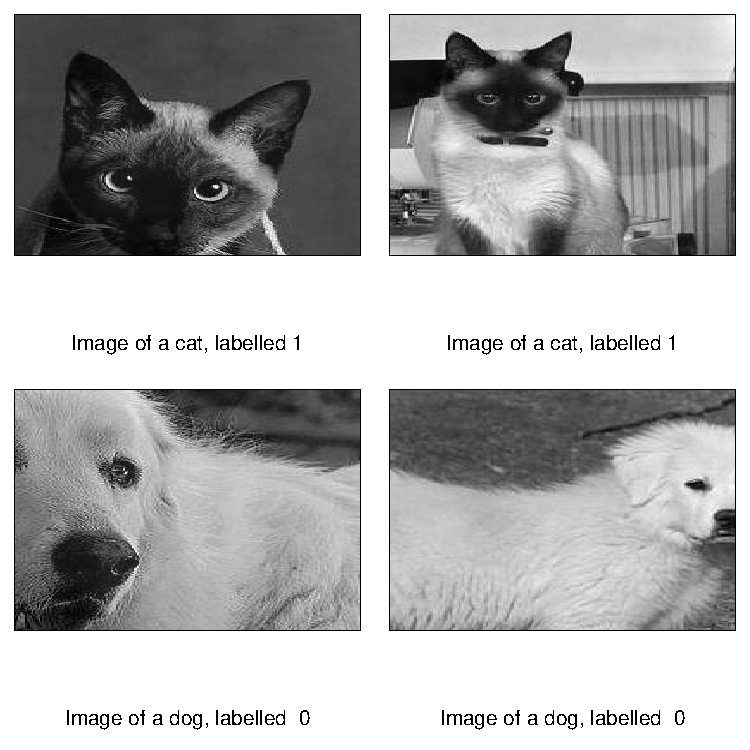
\includegraphics[width=\maxwidth]{figure/unnamed-chunk-2-1} 
\begin{kframe}\begin{verbatim}
## [1] "Percentage of positive targets (cats) in train set"
## [2] "0.498412698412698"
## [1] "Percentage of positive targets (cats) in test set"
## [2] "0.479166666666667"
\end{verbatim}
\end{kframe}
\end{knitrout}

Le label 1 correspond aux images de chats (et donc le label 0 correspond aux chiens), il y a 363 observations dont 315 dans le train set et 48 dans le test set. Il y a 49.8\% de chats dans le train set et 47,9\% dans le test set. Chaque image est représentée comme un vecteur de $\mathbb{R}^{40000}$

\subsection{Question (2)} 

La fonction SVD nous retourne directement la matrice $V$ de la décomposition en valeurs singulières, les 15 premières composantes principales sont ensuite selectionées en conservant les 15 premières colonnes de la matrice de PCA $CV$. La fonction \emph{compute\_PCA} s'occupe du calcul des composantes principales, de découper à nouveaux les données et de sauvegarder les données réduites dans $C_{train}.Rdata$ et $C_{test}.Rdata$ et retourne la variance expliquée (voir ci-dessous).

\begin{knitrout}
\definecolor{shadecolor}{rgb}{0.969, 0.969, 0.969}\color{fgcolor}\begin{kframe}
\begin{alltt}
\hlstd{compute_PCA} \hlkwb{<-} \hlkwa{function}\hlstd{(}\hlkwc{Xtrain}\hlstd{,}\hlkwc{Xtest}\hlstd{) \{}
  \hlstd{X} \hlkwb{=} \hlkwd{rbind}\hlstd{(Xtrain,Xtest)} \hlcom{#concatenation}
  \hlstd{X} \hlkwb{=} \hlkwd{scale}\hlstd{(X,} \hlkwc{center} \hlstd{=} \hlnum{TRUE}\hlstd{,} \hlkwc{scale} \hlstd{=} \hlnum{FALSE}\hlstd{)}  \hlcom{#centrage }
  \hlstd{PCA} \hlkwb{=} \hlkwd{svd}\hlstd{(X,}\hlkwc{nu}\hlstd{=}\hlnum{0}\hlstd{,}\hlkwc{nv}\hlstd{=}\hlnum{15}\hlstd{)} \hlcom{#nv=15 on ne conserve que 15 composantes}
  \hlstd{C} \hlkwb{=} \hlstd{X} \hlopt \hlstd{PCA}\hlopt{$}\hlstd{v}
  \hlstd{Ctrain} \hlkwb{=} \hlstd{C[}\hlnum{1}\hlopt{:}\hlnum{315}\hlstd{,]}
  \hlstd{Ctest} \hlkwb{=} \hlstd{C[}\hlnum{316}\hlopt{:}\hlkwd{dim}\hlstd{(C)[}\hlnum{1}\hlstd{],]}
  \hlkwd{save}\hlstd{(Ctrain,} \hlkwc{file} \hlstd{=} \hlstr{"Ctrain.RData"}\hlstd{)} \hlcom{#sauvegarde des donnees reduites}
  \hlkwd{save}\hlstd{(Ctest,} \hlkwc{file} \hlstd{=} \hlstr{"Ctest.RData"}\hlstd{)}

  \hlkwd{return}\hlstd{(}\hlkwd{sum}\hlstd{(PCA}\hlopt{$}\hlstd{d[}\hlnum{1}\hlopt{:}\hlnum{15}\hlstd{]}\hlopt{**}\hlnum{2}\hlstd{)}\hlopt{/}\hlkwd{sum}\hlstd{(PCA}\hlopt{$}\hlstd{d}\hlopt{**}\hlnum{2}\hlstd{))} \hlcom{#variance expliquee}
\hlstd{\}}
\end{alltt}
\end{kframe}
\end{knitrout}

Soit $\lambda_1 > \cdots > \lambda_{373}$ les valeurs singulières ordonées par ordre décroissant. Le pourcentage de variance expliqué par les 15 premières composantes principales est donné par : \[\frac{\sum_{i=1}^{15} \lambda_i^2}{\sum_{i=1}^{373} \lambda_i^2}\] 

\begin{knitrout}
\definecolor{shadecolor}{rgb}{0.969, 0.969, 0.969}\color{fgcolor}\begin{kframe}
\begin{alltt}
\hlstd{var_expl} \hlkwb{=} \hlkwd{compute_PCA}\hlstd{(Xtrain,Xtest)}
\hlstd{var_expl}
\end{alltt}
\begin{verbatim}
## [1] 0.7134303
\end{verbatim}
\end{kframe}
\end{knitrout}

La fonction \emph{compute\_PCA} retourne un pourcentage de variance expliqué de 71,34\%.

\subsection{Question (3)}

Les notations choisies pour formaliser le modèle statistique sont : \(\mathcal{B}(\mathbb{R}^{15})\) pour la tribu borélienne engendrée par \(\mathbb{R}^{15}\), \(\mathcal{P}(\{0,1\})\) pour l'ensemble des parties de $\{0,1\}$, $\otimes$ represente l'opération produit de tribus \footnote{Soient $\mathcal{A}$ et $\mathcal{B}$ deux tribus, $\mathcal{A} \otimes \mathcal{B}$ est la tribu engendrée par les pavés $A \times B$ où $A \in \mathcal{A}, B \in \mathcal{B}$}, $\mathbb{M}^{a \times b}$ est l'espace des matrices réelles à a lignes et b colonnes. Nous définissons de plus \[\forall B \in \mathcal{B}(\mathbb{R}^{15}), \forall j \in \{0,1\}, m_j(B) = \int_B \frac{1}{(2\pi)^{15/2}}(\det\Sigma_j)^{-1/2}exp\{-\frac{1}{2}(c-\mu_j)^T\Sigma_j^{-1} (c-\mu_j)\}dc\] et \[ \theta = (p, \mu_0, \mu_1, \Sigma_0, \Sigma_1)\]

Le modèle statistique associé aux observations $((c_1,y_1), \ldots, (c_n,y_n))$ est l'espace de probabilité $(\Omega, \mathcal{F}, (\mathbb{P}_{\theta}, \theta \in \Theta))$ donné par  \\
$$
\begin{array}{lcl}
\Omega = (\mathbb{R}^{15} \times \{0,1\})^n \\ \\
\mathcal{F} = (\mathcal{B}(\mathbb{R}^{15}) \otimes \mathcal{P}(\{0,1\}))^{\otimes^n} \\ \\
\Theta = [0,1] \times \mathbb{R}^{15} \times \mathbb{R}^{15} \times \mathbb{M}^{15 \times 15} \times \mathbb{M}^{15 \times 15} \\ \\
\forall \theta \in \Theta, \forall B \in \mathcal{B}(\mathbb{R}^{15}), \forall A \in
\mathcal{P}(\{0,1\}),  \\ \\
~~~~~~~~~~~~ \mathbb{P}_{\theta}(A \times B) = p\delta_1(A) m_1(B) + (1-p)\delta_0(A) m_0(B) \\
\end{array}
$$

\begin{rmq}
On vérifie bien que \(\mathbb{P}_{\theta}(\{0,1\} \times \mathbb{R}^{15}) = p\delta_1(\{0,1\}) \times 1 + (1-p)\delta_0(\{0,1\}) \times 1 = p + 1 - p = 1 \). De plus, en prenant $B = \mathbb{R}^{15}$ on retombe bien sur une loi de Bernouilli de paramètre $p$ pour la loi marginale de Y \[ \mathbb{P}_{\theta}(A \times \mathbb{R}^{15}) = p\delta_1(A) + (1-p)\delta_0(A)\] 
\end{rmq}



\section{Analyse Discriminante Quadratique}

\subsection{Question (4)}

\noindent Par d\'efinition de la vraisemblance on a que 
$$
L((c_1,y_1),\hdots,(c_n,y_n)|\theta) = \prod_{i=1}^n f_{c,Y}(c_i,y_i) = \prod_{i=1}^n f_{Y}(y_i)f_{c|Y_i=y_i}(c)
$$
D\`es lors on a que 
$$
\begin{array}{rcl}
L((c_1,y_1),\hdots,(c_n,y_n)|\theta) & = &  \prod_{i=1}^n \bigg{\{}p^{y_i}(1-p)^{1-y_i} \\ \\
& & \bigg{[}\frac{1}{(2\pi)^{15/2}}(\det\Sigma_1)^{-1/2}exp\{-\frac{1}{2}(c_i-\mu_1)^T\Sigma_1^{-1} (c_i-\mu_1\}\bigg{]}^{\mathbbm{1}_{y_i=1}}  \\
& & \bigg{[}\frac{1}{(2\pi)^{15/2}}(\det\Sigma_0)^{-1/2}exp\{-\frac{1}{2}(c_i-\mu_0)^T\Sigma_0^{-1} (c_i-\mu_0\}\bigg{]}^{\mathbbm{1}_{y_i=0}} \bigg{\}} \\ \\
& = & p^{\sum_i y_i}(1-p)^{n-\sum_i y_i}\\ \\
& & \bigg{[}\frac{1}{(2\pi)^{15/2}}(\det\Sigma_1)^{-1/2}\bigg{]}^{\sum_i y_i}\bigg{[}\frac{1}{(2\pi)^{15/2}}(\det\Sigma_0)^{-1/2}\bigg{]}^{n-\sum_i y_i} \\ \\
& & exp\bigg{\{}-\frac{1}{2}\big{[}\sum_{i,y_i = 1}(c_i-\mu_1)^T\Sigma_1^{-1} (c_i-\mu_1)+\sum_{i,y_i = 0}(c_i-\mu_0)^T\Sigma_0^{-1} (c_i-\mu_0)\big{]}\bigg{\}} \\ \\
& = & p^{N_1}(1-p)^{N_2}\\ \\
& & \bigg{[}\frac{1}{(2\pi)^{15/2}}(\det\Sigma_1)^{-1/2}\bigg{]}^{N_1}\bigg{[}\frac{1}{(2\pi)^{15/2}}(\det\Sigma_0)^{-1/2}\bigg{]}^{N_2} \\ \\
& & exp\bigg{\{}-\frac{1}{2}\big{[}\sum_{i,y_i = 1}(c_i-\mu_1)^T\Sigma_1^{-1} (c_i-\mu_1)+\sum_{i,y_i = 0}(c_i-\mu_0)^T\Sigma_0^{-1} (c_i-\mu_0)\big{]}\bigg{\}} \\
\end{array}
$$
Ainsi, la log-vraisemblance est de la forme,
\begin{equation}
\begin{array}{rcl}
l((c_1,y_1),\hdots,(c_n,y_n)|\theta) & = & \displaystyle{N_1 \log(p) + N_2 \log(1-p) - \frac{N_1}{2}\log(\det(\Sigma_1))}\\ \\
& & \displaystyle{- \frac{1}{2}\sum_{i,y_i = 1}(c_i-\mu_1)^T \Sigma_1^{-1}(c_i-\mu_1) - \frac{N_2}{2}\log(\det(\Sigma_0))} \\ \\
& & \displaystyle{-\frac{1}{2}\sum_{i,y_i = 0}(c_i-\mu_0)^T \Sigma_0^{-1}(c_i-\mu_0) + \mbox{constante}}
\end{array}
\end{equation}

avec $\mbox{constante} = -\frac{15n}{2}log(2\pi)$


\subsection{Question (5)}
\noindent L'estimateur du maximum de vraisemblance pour $p$ est obtenu par la CPO, on a :
$$
\begin{array}{rcl}
\displaystyle{\frac{\partial l((c_1,y_1),\hdots,(c_n,y_n)|\theta)}{\partial p}} & = & 0 \\ \\
\displaystyle{\Leftrightarrow \frac{N_1}{p} - \frac{N_2}{1-p}} & = & 0 \\ \\
\Leftrightarrow (1-p)N_1 & = & N_2 p \\ \\
\Leftrightarrow N_1 & = & (N_1 + N_2) p \\ \\
\Leftrightarrow \hat{p} & = & \displaystyle{\frac{N_1}{n}} \\
\end{array}
$$
Pour $\mu_1$ et $\mu_0$ le calcul est rigoureusement le m\^eme, voici celui pour $\mu_1$ \`a nouveau gr\^ace \`a la CPO : 
$$
\begin{array}{rcl}
\displaystyle{\frac{\partial l((c_1,y_1),\hdots,(c_n,y_n)|\theta)}{\partial\mu_1}} & = & 0 \\ \\
\displaystyle{\Leftrightarrow \frac{\partial}{\partial \mu_1} \sum_{i,y_i = 1}(c_i-\mu_1)^T\Sigma_1^{-1} (c_i-\mu_1)} & = & 0  \\ \\
\displaystyle{\Leftrightarrow \frac{\partial}{\partial \mu_1}\bigg{\{}}\sum_{i,y_i = 1}c_i^T\Sigma_1^{-1}c_i - c_i^T\Sigma_1^{-1}\mu_1 - \mu_1^T\Sigma_1^{-1}c_i + \mu_1^T\Sigma_1^{-1}\mu_1\bigg{\}} & = & 0 \\ \\
\displaystyle{\Leftrightarrow \sum_{i,y_i = 1}(- (c_i^T\Sigma_1^{-1})^T - \Sigma_1^{-1} c_i + \big{(} \Sigma_1^{-1} + (\Sigma_1^{-1})^T \big{)}\mu_1 } & = & 0
\end{array}
$$
En tant que matrice de variance-covariance $\Sigma_1$ et $\Sigma_0$ sont sym\'etriques, il en va de m\^eme pour leur inverse, ainsi $\Sigma_1^{-1} = (\Sigma_1^{-1})^T$ et $\Sigma_0^{-1} = (\Sigma_0^{-1})^T$. D\`es lors,
$$
\begin{array}{rcl}
\displaystyle{\frac{\partial l((c_1,y_1),\hdots,(c_n,y_n)|\theta)}{\partial\mu_1}} & = & 0 \\ \\
\displaystyle{\Leftrightarrow 2\sum_{i,y_i = 1}\Sigma_1^{-1} c_i} & = & \displaystyle{2 N_1\Sigma_1^{-1}\mu_1} \\ \\
\displaystyle{\Leftrightarrow \sum_{i,y_i = 1}\Sigma_1 \Sigma_1^{-1} c_i} & = & N_1 \mu_1 \\ \\
\displaystyle{\Leftrightarrow \hat \mu_1} & = & \displaystyle{\frac{1}{N_1}\sum_{i,y_i = 1} c_i}
\end{array}
$$
De m\^eme, 
$$
\hat \mu_0 =  \frac{1}{N_2}\sum_{i,y_i = 0} c_i
$$
De m\^eme pour $\Sigma_1$ et $\Sigma_0$ les r\'esultats sont rigoureusement identiques, en s'aidant des formules de dérivées matricielles données on a,
$$
\begin{array}{rcl}
\displaystyle{\frac{\partial l((c_1,y_1),\hdots,(c_n,y_n)|\theta)}{\partial\Sigma_1}} & = & 0 \\ \\
\displaystyle{\Leftrightarrow \frac{N_1}{2}\Sigma_1^{-1} -  \frac{1}{2}\sum_{i,y_i=1} \Sigma_1^{-1}(c_i-\mu_1)(c_i-\mu_1)^T\Sigma_1^{-1}} & = & 0 \\ \\
\displaystyle{\Leftrightarrow \frac{1}{N_1}\sum_{i,y_i=1} \Sigma_1^{-1}(c_i-\mu_1)(c_i-\mu_1)^T\Sigma_1^{-1}} & = & \displaystyle{ \Sigma_1^{-1}} \\ \\
\displaystyle{\Leftrightarrow \Sigma_1^{-1}\frac{1}{N_1}\sum_{i,y_i=1}(c_i-\mu_1)(c_i-\mu_1)^T} &= & \displaystyle{I_{15}}
\end{array}
$$

\[ \Leftrightarrow \hat{\Sigma_1} = \frac{1}{N_1}\sum_{i,y_i=1}(c_i-\mu_1)(c_i-\mu_1)^T\]


Ainsi en subtituant les estimateurs de $\mu_1$ et $\mu_0$ on obtient que,
$$
\begin{array}{rcl}
\displaystyle{\hat \Sigma_1} & = & \displaystyle{\frac{1}{N_1}\sum_{i,Y_i=1}(c_i-\hat \mu_1)(c_i-\hat \mu_1)^T} \\ \\
\displaystyle{\hat \Sigma_0} & = & \displaystyle{\frac{1}{N_2}\sum_{i,Y_i=0}(c_i-\hat \mu_0)(c_i-\hat \mu_0)^T}
\end{array}
$$
Les estimateurs du maximum de vraisemblance sont donc :
$$
\left \{
\begin{array}{rcl}
\hat{p} & = & \displaystyle{\frac{N_1}{n}} \\ \\
\displaystyle{\hat \mu_1} & = & \displaystyle{\frac{1}{N_1}\sum_{i,y_i = 1} c_i} \\ \\
\hat \mu_0 & = &  \displaystyle{\frac{1}{N_2}\sum_{i,y_i = 0} c_i} \\ \\
\displaystyle{\hat \Sigma_1} & = & \displaystyle{\frac{1}{N_1}\sum_{i,y_i=1}(c_i-\hat{\mu}_1)(c_i-\hat{\mu}_1)^T} \\ \\
\displaystyle{\hat \Sigma_0} & = & \displaystyle{\frac{1}{N_2}\sum_{i,y_i=0}(c_i-\hat{\mu}_0)(c_i-\hat{\mu}_0)^T}
\end{array}
\right.
$$


\subsection{Question (6)}

\noindent Le sous-gradient $\nabla_{p,\mu_1,\mu_0}l(\theta)$ est de la forme 
$$
\nabla_{p,\mu_0,\mu_1}l(\theta) = 
\begin{pmatrix} 
\frac{N_1}{p} - \frac{N_2}{1-p} \\
-2\sum_{i,y_i = 1}\Sigma_1^{-1} c_i + \Sigma_1^{-1}\mu_1 \\
-2\sum_{i,y_i = 0}\Sigma_1^{-1} c_i + \Sigma_1^{-1}\mu_0
\end{pmatrix}
$$

\begin{rmq}
\(\nabla_{p,\mu_1,\mu_0}l(\theta) \in \mathbbm{R}^{15}\)
\end{rmq}

Par cons\'equent on obtient la sous-hessienne suivante
$$
\nabla_{p,\mu_0,\mu_1}^2l(\theta) = 
\begin{pmatrix} 
-\frac{N_1}{p^2} - \frac{N_2}{(1-p)^2} & 0_{\mathbb{M}^{1 \times 15}} & 0_{\mathbb{M}^{1 \times 15}} \\
0_{\mathbbm{R}^{15}} & -2 N_1\Sigma_1^{-1}& 0_{\mathbb{M}^{15 \times 15}} \\
0_{\mathbbm{R}^{15}} & 0_{\mathbb{M}^{15 \times 15}} & -2 N_1\Sigma_0^{-1}
\end{pmatrix}
$$
La matrice est diagonale par blocs et chacun de ses blocs est défini négatif. En effet, nous savons que les matrices de covariances $\Sigma_0$ et $\Sigma_1$ sont définies positives donc leur inverse aussi et donc $-2 N_1\Sigma_0^{-1}$ et $-2 N_1\Sigma_1^{-1}$ sont définies négatives. C'est un exercice facile mais fastidieux à rédiger de voir que si la matrice est diagonale par blocs avec chacun de ses blocs défini négatif alors la matrice entière est définie négative.

\begin{rmq}
\(\nabla_{p,\mu_0,\mu_1}^2l(\theta) \in \mathbb{M}^{31 \times 31}\)
\end{rmq}

\subsection{Question (7)}
$$
\mathbb{E}[\hat p]= \mathbb{E}\bigg{[}\frac{\sum_{i=1}^n y_i}{n}\bigg{]} = \frac{1}{n}\sum_i \mathbb{E}[y_i] = \mathbb{E}[y_1] = p
$$

$$
\begin{array}{rcl}
\mathbb{E}[\hat \mu_1] & = & \mathbb{E}\bigg{[} \mathbb{E}[\hat \mu_1 |y_1, \hdots , y_n] \bigg{]} = 
\mathbb{E}\bigg{[}\frac{1}{N_1} \mathbb{E}\bigg{[}\sum_{i} c_i \mathbbm{1}_{y_i=1} \bigg{|}y_1, \hdots , y_n \bigg{]} \bigg{]} \\ \\
& = & \mathbb{E}\bigg{[}\frac{1}{N_1} \sum_{i} \mathbbm{1}_{y_i=1} \mathbb{E}\bigg{[} c_i  \bigg{|}y_1, \hdots , y_n \bigg{]} \bigg{]} = \mathbb{E}\bigg{[}\frac{1}{N_1} \sum_{i} \mathbbm{1}_{y_i=1} \mathbb{E}[ c_i  | y_i ] \bigg{]} 
\end{array}
$$
Ici nous avons utilisé l'indépendance de $(c_i,y_i)$ avec $(y_j)_{j \neq i}$ ce qui permet d'obtenir $\mathbb{E}[ c_i  |y_1, \hdots , y_n ] = \mathbb{E}[ c_i  | y_i ]$ \footnote{Pour une preuve rigoureuse de ce résultat voir \emph{Probability with Martingales} de David Williams, page 88 : proposition (k) "Role of Independence"}, or $\mathbb{E}[ c_i  | y_i ] \mathbbm{1}_{y_i=1} = \mu_1 \mathbbm{1}_{y_i=1}$, on obtient donc \[ \mathbb{E}[\hat \mu_1] = \mathbb{E}\bigg{[}\frac{1}{N_1}\sum_{i} \mathbbm{1}_{y_i=1} \mu_1 \bigg{]} = \mu_1 \mathbb{E}[\frac{N_1}{N_1}] = \mu_1 \]

De même, en effectuant exactement le même calcul pour $\mu_0$ : 

$$
\mathbb{E}[\hat \mu_0]  = \mu_0
$$

\subsection{Question (8)}
On a que $\mathbb{E}[Y] = p$, d\`es lors l'estimateur de la m\'ethode des moments qui est l'équivalent empirique de $\mathbb{E}[Y]$ est
$$
p^{MM} = \bar Y = \frac{1}{n} \sum_i y_i = \frac{N_1}{n} = \hat p
$$
De m\^eme on a que $\mathbb{E}[C|Y=1] = \mu_1$, avec, 
$$
\mathbb{E}[C|Y=1]= \frac{\mathbb{E}[C\mathbbm{1}\{Y=1\}]}{\mathbb{E}[\mathbbm{1}\{Y=1\}]}
$$
ainsi l'estimateur de la m\'ethode des moments est l'équivalent empirique de cette quantité :
$$
\mu_1^{MM}=\frac{\frac{1}{n}\sum_{i=1}^n c_i \mathbbm{1}_{y_i=1}}{\frac{1}{n}\sum_{i=1}^n \mathbbm{1}_{y_i=1}} = \frac{\sum_{i,y_i=1}c_i}{\sum_{i}y_i} = \frac{\sum_{i,y_i=1}c_i}{N_1} = \hat \mu_1
$$
De m\^eme on a que $\mathbb{E}[C|Y=0] = \mu_0$, ainsi l'estimateur de la m\'ethode des moments est le moment empirique de 
$$
\mathbb{E}[C|Y=0]= \frac{\mathbb{E}[C\mathbbm{1}\{Y=0\}]}{\mathbb{E}[\mathbbm{1}\{Y=0\}]}
$$
\`a savoir 
$$
\mu_0^{MM}=\frac{\frac{1}{n}\sum_{i,y_i=0}c_i}{\frac{1}{n}\sum_{i,y_i=0}y_i}= \frac{\sum_{i,y_i=1}c_i}{\sum_{i}(1-y_i)} = \frac{\sum_{i,y_i=1}c_i}{N_2} = \hat \mu_0
$$
Enfin, on a que $\mathbb{V}(C|Y=1) = \Sigma_1$, l'estimateur de la m\'ethode des moments est donc le moment empirique de 
$$
\mathbb{V}(C|Y=1) = \mathbb{E}[(c-\mu_1)(c-\mu_1)^T|Y=1]
$$
\`a savoir, en se servant des estimateurs de $\mu_0$ et $\mu_1$ : 
$$
\Sigma_1^{MM}= \frac{1}{N_1}\sum_{i,y_i=1}(c_i-\hat{\mu}_1)(c_i-\hat{\mu}_1)^T = \hat \Sigma_1
$$ 
De m\^eme pour $\Sigma_0^{MM}$,
$$
\Sigma_0^{MM}= \frac{1}{N_2}\sum_{i,y_i=0}(c_i-\hat{\mu}_0)(c_i-\hat{\mu}_0)^T = \hat \Sigma_0
$$

\subsection{Question (9)}

La fonction \emph{computeML} se charge de calculer les estimateurs déterminés à la question 5. Nous avons ensuite comparé les résultats obtenus avec ceux de la fonction \emph{qda} du package \emph{MASS}. On oberve uniquement une légère différence sur les valeurs des log de déterminant. Ces erreurs viennent probablement d'approximations numériques et de la façon de calculer les déterminants.

\begin{knitrout}
\definecolor{shadecolor}{rgb}{0.969, 0.969, 0.969}\color{fgcolor}\begin{kframe}
\begin{alltt}
\hlkwd{load}\hlstd{(}\hlstr{"Ctrain.RData"}\hlstd{)}
\hlkwd{load}\hlstd{(}\hlstr{"Ctest.RData"}\hlstd{)}

\hlstd{computeML} \hlkwb{<-} \hlkwa{function}\hlstd{(}\hlkwc{C}\hlstd{,} \hlkwc{Y}\hlstd{)\{}
  \hlstd{n} \hlkwb{=} \hlkwd{length}\hlstd{(Y)}
  \hlstd{N1} \hlkwb{=} \hlkwd{sum}\hlstd{(Y}\hlopt{==}\hlnum{1}\hlstd{)}
  \hlstd{C0} \hlkwb{=} \hlstd{C[Y}\hlopt{==}\hlnum{0}\hlstd{,]}
  \hlstd{C1} \hlkwb{=} \hlstd{C[Y}\hlopt{==}\hlnum{1}\hlstd{,]}

  \hlstd{p_hat} \hlkwb{=} \hlstd{N1}\hlopt{/}\hlstd{n}
  \hlstd{mu_hat0} \hlkwb{=} \hlkwd{colMeans}\hlstd{(C0)}
  \hlstd{mu_hat1} \hlkwb{=} \hlkwd{colMeans}\hlstd{(C1)}
  \hlstd{C0_centered} \hlkwb{=} \hlkwd{sweep}\hlstd{(C0,}\hlnum{2}\hlstd{,mu_hat0)} \hlcom{#susbtract mu_hat0 to C0 }
  \hlstd{C1_centered} \hlkwb{=} \hlkwd{sweep}\hlstd{(C1,}\hlnum{2}\hlstd{,mu_hat1)}
  \hlstd{sigma_hat0} \hlkwb{=} \hlkwd{t}\hlstd{(C0_centered)}\hlopt\hlstd{C0_centered}\hlopt{/}\hlstd{(n}\hlopt{-}\hlstd{N1)}
  \hlstd{sigma_hat1} \hlkwb{=} \hlkwd{t}\hlstd{(C1_centered)}\hlopt\hlstd{C1_centered}\hlopt{/}\hlstd{N1}

  \hlstd{out} \hlkwb{=} \hlkwd{list}\hlstd{(p_hat,mu_hat0,mu_hat1,sigma_hat0,sigma_hat1)}

  \hlkwd{return}\hlstd{(out)}
\hlstd{\}}

\hlstd{ML} \hlkwb{=} \hlkwd{computeML}\hlstd{(Ctrain,Ytrain)}

\hlcom{#QDA from MASS package}
\hlstd{qda.model} \hlkwb{=} \hlkwd{qda}\hlstd{(Ctrain,Ytrain)}
\end{alltt}
\end{kframe}
\end{knitrout}

\begin{knitrout}
\definecolor{shadecolor}{rgb}{0.969, 0.969, 0.969}\color{fgcolor}\begin{kframe}
\begin{verbatim}
## Estimation of p :  0.4984127
## QDA estimation of p :  0.4984127
## Estimation of log(det(sigma0)) :  102.7835
## QDA estimation of log(det(sigma0)) :  102.8787
## Estimation of log(det(sigma1)) :  105.5119
## QDA estimation of log(det(sigma1)) :  105.6077
## Estimation of mu0[1:4] :  51.136 4.886618 0.9851159 10.69928
## QDA estimation of mu0[1:4] :  51.136 4.886618 0.9851159 10.69928
## Estimation of mu1[1:4] :  -52.21073 -2.780416 0.3652852 -11.93721
## QDA estimation of mu1[1:4] :  -52.21073 -2.780416 0.3652852 -11.93721
\end{verbatim}
\end{kframe}
\end{knitrout}

\subsection{Question (10)}

Soit $j \in \{0,1\}$, d'après la formule de Bayes (appliquée deux fois),
\[\mathbb{P} (Y=j| c) = \frac{f_{C,Y}(c,j)}{f_C(c)} = \frac{\mathbb{P} (Y=j)f_{C|Y=j}(c)}{f_C(c)}\]
Comme $C|Y=j \sim N(\mu_j, \Sigma_j)$ et  $\mathbb{P} (Y=j) = p^j(1-p)^{1-j}$ et 
\[f_C(c) = \int f_{C,Y}(c,j) d_{\mu}(j)) = f_{C|Y=0}(c)\mathbb{P} (Y=0) + f_{C|Y=1}(c)\mathbb{P} (Y=1) = (1-p)\varphi(c; \mu_0, \Sigma_0) + p\varphi(c; \mu_1, \Sigma_1)\] avec $\mu$ la mesure de comptage, on obtient : 

\[ \mathbb{P} (Y=1| c) = \frac{p\varphi(c; \mu_1, \Sigma_1)}{(1-p)\varphi(c; \mu_0, \Sigma_0) + p\varphi(c; \mu_1, \Sigma_1)}\]
\[ \mathbb{P} (Y=0| c) = \frac{(1-p)\varphi(c; \mu_0, \Sigma_0)}{(1-p)\varphi(c; \mu_0, \Sigma_0) + p\varphi(c; \mu_1, \Sigma_1)}\]

\subsection{Question (11)}

On observe que le terme de normalisation $m=(1-p)\varphi(c; \mu_0, \Sigma_0) + p\varphi(c; \mu_1, \Sigma_1)$ va se simplifier lorqu'on fait le ratio des deux quantités : \[\frac{\mathbb{P} (Y=1| c)}{\mathbb{P} (Y=0| c)} = \frac{p\varphi(c; \mu_1, \Sigma_1)}{(1-p)\varphi(c; \mu_0, \Sigma_0)}\]
En passant en log on obtient : 

$$
\begin{array}{rcl}
\log \bigg{\{}\frac{\mathbb{P} (Y=1| c)}{\mathbb{P} (Y=0| c)} \bigg{\}} & = & \log(p) - \log(1-p) + \log(\varphi(c; \mu_1, \Sigma_1)) - \log(\varphi(c; \mu_0, \Sigma_0))  \\ \\ 
& = & \log(p) - \log(1-p) - \frac{1}{2}\log(\det(\Sigma_1)) + \frac{1}{2}\log(\det(\Sigma_0)) \\ \\ & & - \frac{1}{2}(c-\mu_1)^T \Sigma_1^{-1}(c-\mu_1) + \frac{1}{2}(c-\mu_0)^T \Sigma_0^{-1}(c-\mu_0) + \frac{15}{2}log(2\pi) - \frac{15}{2}log(2\pi) \\ \\ & = & - \frac{1}{2}\log(\det(\Sigma_1)) - \frac{1}{2}(c-\mu_1)^T \Sigma_1^{-1}(c-\mu_1) + \log(p) \\ \\ & & + \frac{1}{2}\log(\det(\Sigma_0)) + \frac{1}{2}(c-\mu_0)^T \Sigma_0^{-1}(c-\mu_0) - \log(1-p)
\end{array}
$$
On obtient bien le résultat souhaité.

\subsection{Question (12)} 

Soit $A$ l'évènement tel que : \[A = \bigg{\{} \log \bigg{(}\frac{\mathbb{P} (Y=1| c)}{\mathbb{P} (Y=0| c)} \bigg{)} > 0  \bigg{\}} = \bigg{\{} \frac{\mathbb{P} (Y=1| c)}{\mathbb{P} (Y=0| c)} > 1 \bigg{\}} = \bigg{\{} \mathbb{P} (Y=1| c) > \mathbb{P} (Y=0| c) \bigg{\}} \]
Donc si $\mathbbm{1}_A = 1$, $A$ est réalisé et $\argmax_{y\in \{0,1\}} \mathbb{P} (Y=y| c) = 1$ et si $\mathbbm{1}_A = 0$ alors $A^c$ est réalisé et $\argmax_{y\in \{0,1\}} \mathbb{P} (Y=y| c) = 0$. Dans tous les cas nous avons bien : 
\[ \mathbbm{1}_{\{ \log (\frac{\mathbb{P} (Y=1| c)}{\mathbb{P} (Y=0| c)} ) > 0\}} = \argmax_{y\in \{0,1\}} \mathbb{P} (Y=y| c) \]

\begin{rmq}
La règle de décision qui en dècoule est bien une fonction \textbf{quadratique} de l'observation $c$ ce qui a donné son nom à la méthode.
\end{rmq}

\subsection{Question (13)}

Soit $x,y \in \{0,1\}$, on a alors quatre cas possibles : 
\begin{itemize}
\item $x=0, y=0$ donne $(x-y)^2 = |x-y| = \mathbbm{1}_{x\neq y} = 0$
\item $x=1, y=1$ donne $(x-y)^2 = |x-y| = \mathbbm{1}_{x\neq y} = 0$
\item $x=0, y=1$ donne $(x-y)^2 = |x-y| = \mathbbm{1}_{x\neq y} = 1$
\item $x=1, y=0$ donne $(x-y)^2 = |x-y| = \mathbbm{1}_{x\neq y} = 1$ \\
Cela implique que si X et Y sont deux variables aleatoires à valeur dans  $\{0,1\}$ alors \[(X-Y)^2 = |X-Y| = \mathbbm{1}_{X=Y} p.s\]
Comme \(\mathbb{E}[\mathbbm{1}_{y=\hat{y}}] = \mathbb{P}(y = \hat{y})\) et $(\hat{y},y) \in \{0,1\}^2$, en passant à l'espérance on obtient bien \[\mathbb{E}[(y-\hat{y})^2] = \mathbb{E}[|y-\hat{y}|] = \mathbb{P}(y = \hat{y})\]

\end{itemize}

\subsection{Question (14)}

La fonction \emph{computeLogRatio} prend en entrée une observation (un vecteur de $\mathbb{R}^{15}$) et les statistiques de la question 5 afin de calculer le log ratio associé à l'observation.

La fonction \emph{computePred} prend en entrée une matrice d'observations et effectue pour chaque observation une prédiction selon la règle de décision de la question 12: le label prédit est 1 si le log ratio est positif et 0 sinon.

\begin{knitrout}
\definecolor{shadecolor}{rgb}{0.969, 0.969, 0.969}\color{fgcolor}\begin{kframe}
\begin{alltt}
\hlstd{computeLogRatio} \hlkwb{<-} \hlkwa{function}\hlstd{(}\hlkwc{cvect}\hlstd{,}\hlkwc{p}\hlstd{,}\hlkwc{mu0}\hlstd{,}\hlkwc{mu1}\hlstd{,}\hlkwc{Sigma0}\hlstd{,}\hlkwc{Sigma1}\hlstd{) \{}

  \hlstd{logratio} \hlkwb{=} \hlstd{(}\hlnum{0.5}\hlopt{*}\hlstd{(}\hlopt{-}\hlkwd{log}\hlstd{(}\hlkwd{det}\hlstd{(Sigma1))} \hlopt{+} \hlkwd{log}\hlstd{(}\hlkwd{det}\hlstd{(Sigma0))}
                  \hlopt{-} \hlkwd{t}\hlstd{(cvect}\hlopt{-}\hlstd{mu1)}\hlopt\hlkwd{ginv}\hlstd{(Sigma1)}\hlopt\hlstd{(cvect}\hlopt{-}\hlstd{mu1)}
                  \hlopt{+} \hlkwd{t}\hlstd{(cvect}\hlopt{-}\hlstd{mu0)}\hlopt\hlkwd{ginv}\hlstd{(Sigma0)}\hlopt\hlstd{(cvect}\hlopt{-}\hlstd{mu0))}
              \hlopt{+} \hlkwd{log}\hlstd{(p)} \hlopt{-} \hlkwd{log}\hlstd{(}\hlnum{1}\hlopt{-}\hlstd{p))}

  \hlkwd{return}\hlstd{(logratio)}
\hlstd{\}}

\hlstd{computePred} \hlkwb{<-} \hlkwa{function}\hlstd{(}\hlkwc{C}\hlstd{,}\hlkwc{p}\hlstd{,}\hlkwc{mu0}\hlstd{,}\hlkwc{mu1}\hlstd{,}\hlkwc{Sigma0}\hlstd{,}\hlkwc{Sigma1}\hlstd{) \{}

  \hlstd{toapply} \hlkwb{<-} \hlkwa{function}\hlstd{(}\hlkwc{cvect}\hlstd{,}\hlkwc{p}\hlstd{,}\hlkwc{mu0}\hlstd{,}\hlkwc{mu1}\hlstd{,}\hlkwc{Sigma0}\hlstd{,}\hlkwc{Sigma1}\hlstd{) \{}
    \hlkwd{return}\hlstd{(}\hlkwd{as.integer}\hlstd{((}\hlkwd{computeLogRatio}\hlstd{(cvect,p,mu0,mu1,Sigma0,Sigma1)}\hlopt{>}\hlnum{0}\hlstd{)))}
  \hlstd{\}}

  \hlstd{pred} \hlkwb{=} \hlkwd{apply}\hlstd{(C,} \hlkwc{MARGIN} \hlstd{=} \hlnum{1}\hlstd{,} \hlkwc{FUN} \hlstd{= toapply,} \hlkwc{p} \hlstd{= p,} \hlkwc{mu0} \hlstd{= mu0,}
               \hlkwc{mu1} \hlstd{= mu1,} \hlkwc{Sigma0} \hlstd{= Sigma0,} \hlkwc{Sigma1} \hlstd{= Sigma1)}

  \hlkwd{return}\hlstd{(pred)}
\hlstd{\}}
\end{alltt}
\end{kframe}
\end{knitrout}

\subsection{Question (15)}

À l'aide des fonctions des questions précédentes, les prédictions se font aisément comme le montre les deux lignes de codes ci-dessous. L'erreur sur le test set est de 12,5\%.

\begin{knitrout}
\definecolor{shadecolor}{rgb}{0.969, 0.969, 0.969}\color{fgcolor}\begin{kframe}
\begin{alltt}
\hlstd{stats} \hlkwb{=} \hlkwd{computeML}\hlstd{(Ctrain,Ytrain)}
\hlstd{prediction} \hlkwb{=} \hlkwd{computePred}\hlstd{(Ctest,stats[[}\hlnum{1}\hlstd{]],stats[[}\hlnum{2}\hlstd{]],stats[[}\hlnum{3}\hlstd{]],stats[[}\hlnum{4}\hlstd{]],stats[[}\hlnum{5}\hlstd{]])}

\hlstd{prediction}
\end{alltt}
\begin{verbatim}
##  [1] 1 1 1 1 1 1 1 1 0 1 0 1 1 0 1 1 1 1 1 1 1 1 1 1 0 0 1 0 0 0 0 0 0 0 0
## [36] 0 0 0 0 0 0 0 0 0 0 0 1 0
\end{verbatim}
\begin{alltt}
\hlcom{#Erreur de prediction :}
\hlkwd{sum}\hlstd{(prediction}\hlopt{==}\hlstd{Ytest)}\hlopt{/}\hlkwd{length}\hlstd{(Ytest)}
\end{alltt}
\begin{verbatim}
## [1] 0.875
\end{verbatim}
\end{kframe}
\end{knitrout}

Nous comparons ces résultats avec ceux fournies par la fonction \emph{qda}:

\begin{knitrout}
\definecolor{shadecolor}{rgb}{0.969, 0.969, 0.969}\color{fgcolor}\begin{kframe}
\begin{alltt}
\hlstd{computeQDA} \hlkwb{<-} \hlkwa{function}\hlstd{(}\hlkwc{Ctrain}\hlstd{,} \hlkwc{Ctest}\hlstd{,} \hlkwc{Ytrain}\hlstd{,} \hlkwc{Ytest}\hlstd{)\{}
  \hlstd{qda.model} \hlkwb{=} \hlkwd{qda}\hlstd{(Ctrain,Ytrain)}
  \hlstd{pred} \hlkwb{=} \hlkwd{predict}\hlstd{(qda.model, Ctest)}
  \hlkwd{print}\hlstd{(pred}\hlopt{$}\hlstd{class)}
  \hlkwd{return}\hlstd{(}\hlkwd{sum}\hlstd{(pred}\hlopt{$}\hlstd{class}\hlopt{==}\hlstd{Ytest)}\hlopt{/}\hlkwd{length}\hlstd{(Ytest))}
\hlstd{\}}

\hlkwd{computeQDA}\hlstd{(Ctrain, Ctest, Ytrain, Ytest)}
\end{alltt}
\begin{verbatim}
##  [1] 1 1 1 1 1 1 1 1 0 1 0 1 1 0 1 1 1 1 1 1 1 1 1 1 0 0 1 0 0 0 0 0 0 0 0
## [36] 0 0 0 0 0 0 0 0 0 0 0 1 0
## Levels: 0 1
## [1] 0.875
\end{verbatim}
\end{kframe}
\end{knitrout}

Les prédictions sont exactement les mêmes et donc le pourcentage d'erreur aussi. Comme vu question 9 ce résultat était attendu car seuls d'infimes écarts surgissaient entre les estimations des log de déterminant. 

Il y a environ 50\% de chats et 50\% de chiens dans le test set donc si on considère le prédicteur aléatoire qui consisterait à tirer à pile ou face chaque prédiction, il ne ferait pas mieux que 50\%. Nous atteignons ici un précision de 87.5\% ce qui est beaucoup plus raisonnable.

\subsection{Bonus, Analyse Discriminante Linéaire}

Dans \emph{The Elements of Statistical Learning} est abordée l'Analyse Discriminante Linéaire, la seule différence avec l'Analyse Discriminante Quadratique est que l'on fait une hypothèse d'\textbf{homoscédacticité} i.e. les deux groupes ont la même variance $\Sigma$ (mais toujours des moyennes $\mu_0$ et $\mu_1$ différentes). Les estimateurs de $\hat{p}$, $\hat{\mu}_0$ et $\hat{\mu}_1$ restent les mêmes et celui de $\Sigma$ est donné par : \[\hat{\Sigma} =  \frac{\sum_{i,y_i=0}(c_i-\hat{\mu}_0)(c_i-\hat{\mu}_0)^T + \sum_{i,y_i=1}(c_i-\hat{\mu}_1)(c_i-\hat{\mu}_1)^T}{n-2} \] 
Le log ratio prend alors une forme légèrement différente : 

\[\log \bigg{(}\frac{\mathbb{P} (Y=1| c)}{\mathbb{P} (Y=0| c)} \bigg{)} = \log(\frac{\hat{p}}{1-\hat{p}}) - \frac{1}{2}(\hat{\mu}_1 + \hat{\mu}_0)^T\hat{\Sigma}^{-1}(\hat{\mu}_1 - \hat{\mu}_0) + c^T \hat{\Sigma}^{-1}(\hat{\mu}_1 - \hat{\mu}_0)\]

La règle de décision est ensuite la même, le label prédit est 1 si cette quantité est positive et 0 sinon. On observe que la règle de décision est maintenant \textbf{linéaire} en l'observation $c$ et non \textbf{quadratique} comme dans les questions précédentes (d'où la différence de nom entre les deux méthodes). À l'aide des fonctions ci-dessous nous conduisons une prédiction sur la base de test avec deux algorithmes d'analyse discriminante linéaire : notre algorithme "maison" et l'algorithme \emph{lda} du package \emph{MASS}.  

\begin{knitrout}
\definecolor{shadecolor}{rgb}{0.969, 0.969, 0.969}\color{fgcolor}\begin{kframe}
\begin{alltt}
\hlstd{computeMLlin} \hlkwb{<-} \hlkwa{function}\hlstd{(}\hlkwc{C}\hlstd{,} \hlkwc{Y}\hlstd{)\{}
  \hlcom{#Calcul les statistiques associees a la LDA}
  \hlstd{n} \hlkwb{=} \hlkwd{length}\hlstd{(Y)}
  \hlstd{N1} \hlkwb{=} \hlkwd{sum}\hlstd{(Y}\hlopt{==}\hlnum{1}\hlstd{)}
  \hlstd{C0} \hlkwb{=} \hlstd{C[Y}\hlopt{==}\hlnum{0}\hlstd{,]}
  \hlstd{C1} \hlkwb{=} \hlstd{C[Y}\hlopt{==}\hlnum{1}\hlstd{,]}
  \hlstd{p_hat} \hlkwb{=} \hlstd{N1}\hlopt{/}\hlstd{n}
  \hlstd{mu_hat0} \hlkwb{=} \hlkwd{colMeans}\hlstd{(C0)}
  \hlstd{mu_hat1} \hlkwb{=} \hlkwd{colMeans}\hlstd{(C1)}
  \hlstd{C0_centered} \hlkwb{=} \hlkwd{sweep}\hlstd{(C0,}\hlnum{2}\hlstd{,mu_hat0)}
  \hlstd{C1_centered} \hlkwb{=} \hlkwd{sweep}\hlstd{(C1,}\hlnum{2}\hlstd{,mu_hat1)}
  \hlstd{Sigma} \hlkwb{=} \hlstd{(}\hlkwd{t}\hlstd{(C0_centered)}\hlopt\hlstd{C0_centered} \hlopt{+} \hlkwd{t}\hlstd{(C1_centered)}\hlopt\hlstd{C1_centered)}\hlopt{/}\hlstd{(n}\hlopt{-}\hlnum{2}\hlstd{)}

  \hlstd{out} \hlkwb{=} \hlkwd{list}\hlstd{(p_hat,mu_hat0,mu_hat1,Sigma)}
  \hlkwd{return}\hlstd{(out)}
\hlstd{\}}

  \hlstd{computeLogRatiolin} \hlkwb{<-} \hlkwa{function}\hlstd{(}\hlkwc{c}\hlstd{,}\hlkwc{p}\hlstd{,}\hlkwc{mu0}\hlstd{,}\hlkwc{mu1}\hlstd{,} \hlkwc{Sigma}\hlstd{) \{}
    \hlcom{#Calcul les log ratio associees a la LDA }

    \hlstd{logratio} \hlkwb{=} \hlstd{(}\hlkwd{log}\hlstd{(p)} \hlopt{-} \hlkwd{log}\hlstd{(}\hlnum{1}\hlopt{-}\hlstd{p)} \hlopt{-} \hlnum{0.5}\hlopt{*}\hlkwd{t}\hlstd{(mu1} \hlopt{+} \hlstd{mu0)}\hlopt\hlkwd{ginv}\hlstd{(Sigma)}\hlopt\hlstd{(mu1} \hlopt{-} \hlstd{mu0)}
                \hlopt{+} \hlkwd{t}\hlstd{(c)}\hlopt\hlkwd{ginv}\hlstd{(Sigma)}\hlopt \hlstd{(mu1}\hlopt{-}\hlstd{mu0))}

    \hlkwd{return}\hlstd{(logratio)}
  \hlstd{\}}

\hlstd{computePredlin} \hlkwb{<-} \hlkwa{function}\hlstd{(}\hlkwc{C}\hlstd{,}\hlkwc{p}\hlstd{,}\hlkwc{mu0}\hlstd{,}\hlkwc{mu1}\hlstd{,}\hlkwc{Sigma}\hlstd{) \{}

  \hlstd{nbobs} \hlkwb{=} \hlkwd{dim}\hlstd{(C)[}\hlnum{1}\hlstd{]}
  \hlstd{pred} \hlkwb{=} \hlkwd{rep}\hlstd{(}\hlnum{0}\hlstd{,nbobs)}
  \hlkwa{for} \hlstd{(i} \hlkwa{in} \hlnum{1}\hlopt{:}\hlstd{nbobs) \{}

    \hlstd{logratio} \hlkwb{=} \hlkwd{computeLogRatiolin}\hlstd{(C[i,],p,mu0,mu1,Sigma)}
    \hlstd{predi} \hlkwb{=} \hlstd{logratio}\hlopt{>}\hlnum{0}
    \hlstd{pred[i]} \hlkwb{=} \hlstd{predi}
  \hlstd{\}}

  \hlkwd{return}\hlstd{(pred)}
\hlstd{\}}

\hlstd{computeLDA} \hlkwb{<-} \hlkwa{function}\hlstd{(}\hlkwc{Ctrain}\hlstd{,} \hlkwc{Ctest}\hlstd{,} \hlkwc{Ytrain}\hlstd{,} \hlkwc{Ytest}\hlstd{)\{}
  \hlstd{lda.model} \hlkwb{=} \hlkwd{lda}\hlstd{(Ctrain,Ytrain)}
  \hlstd{pred} \hlkwb{=} \hlkwd{predict}\hlstd{(lda.model, Ctest)}
  \hlkwd{print}\hlstd{(pred}\hlopt{$}\hlstd{class)}
  \hlkwd{return}\hlstd{(}\hlkwd{sum}\hlstd{(pred}\hlopt{$}\hlstd{class}\hlopt{==}\hlstd{Ytest)}\hlopt{/}\hlkwd{length}\hlstd{(Ytest))}
\hlstd{\}}


\hlstd{statsbis} \hlkwb{=} \hlkwd{computeMLlin}\hlstd{(Ctrain,Ytrain)}
\hlstd{prediction} \hlkwb{=} \hlkwd{computePredlin}\hlstd{(Ctest,statsbis[[}\hlnum{1}\hlstd{]],statsbis[[}\hlnum{2}\hlstd{]],statsbis[[}\hlnum{3}\hlstd{]],statsbis[[}\hlnum{4}\hlstd{]])}
\hlstd{prediction}
\end{alltt}
\begin{verbatim}
##  [1] 1 0 1 1 1 0 1 1 1 1 0 1 0 0 1 1 1 1 1 1 1 0 0 0 0 0 0 0 0 0 0 0 0 0 0
## [36] 0 0 0 1 0 0 1 0 0 0 0 0 0
\end{verbatim}
\begin{alltt}
\hlkwd{sum}\hlstd{(prediction}\hlopt{==}\hlstd{Ytest)}\hlopt{/}\hlkwd{length}\hlstd{(Ytest)}
\end{alltt}
\begin{verbatim}
## [1] 0.8125
\end{verbatim}
\begin{alltt}
\hlkwd{computeLDA}\hlstd{(Ctrain, Ctest, Ytrain, Ytest)}
\end{alltt}
\begin{verbatim}
##  [1] 1 0 1 1 1 0 1 1 1 1 0 1 0 0 1 1 1 1 1 1 1 0 0 0 0 0 0 0 0 0 0 0 0 0 0
## [36] 0 0 0 1 0 0 1 0 0 0 0 0 0
## Levels: 0 1
## [1] 0.8125
\end{verbatim}
\end{kframe}
\end{knitrout}

Comme pour l'Analyse Discriminante Quadratique ici nos résultats sont exactement les mêmes que ceux de la fonction \emph{lda}. Les hypothèses de l'Analyse Discriminante Linéaire sont plus fortes et on observe une augmentation du taux d'erreur, on passe de 12,5\% d'erreur à 18.75\% d'erreur.


\end{document}



